\documentclass[a4paper]{article}
\usepackage{INTERSPEECH2016}
\usepackage{graphicx}
\usepackage{dblfloatfix}
\usepackage[superscript,biblabel]{cite}
\newcommand\independent{\protect\mathpalette{\protect\independenT}{\perp}}
\def\independenT#1#2{\mathrel{\rlap{$#1#2$}\mkern2mu{#1#2}}}
\title{Establishing Causality in Microbiome/Disease Interactions\\A
  Study in Crohn's Disease}
%\subtitle{A Study in Crohn's Disease}
\name{Daniel Speyer}
\address{dls2192@columbia.edu}
\begin{document}
\ninept

%\twocolumn[
%  \begin{@twocolumnfalse}
    \maketitle
%  \end{@twocolumnfalse}
%]

\begin{abstract}
The literature abounds with correlational studies matching diseases to
gut microbiome dysbiosis, but medical practice does not abound with
corresponding probiotic therapies.  One critical missing piece is
causality.  If the dysbiosis is a \textit{result} of the disease,
then there is no point in correcting the dysbiosis.  In this paper we
present three statistical techniques for determining causality from
existing data and apply them to Crohn's Disease.  The first technique
is to find bacteria which are the mechanism by which a gene causes the
disease.  The second is to find bacteria that correlate to the
disease, but not to that gene.  The final technique is to look for a
specific three-species motif, with a distinctive set of conditional
dependences and independences.
\end{abstract}

\begin{figure*}[t]
  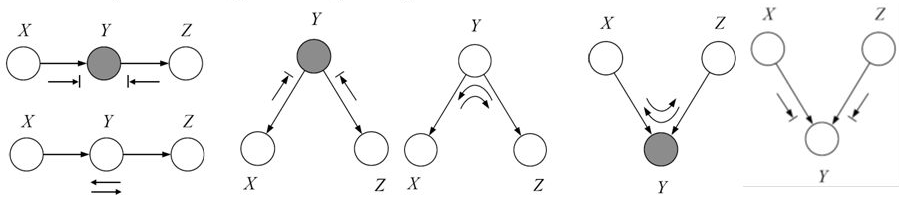
\includegraphics[width=\textwidth]{bayesball}
  \caption{The ``Bayes Ball'' rule: how mutual information travels and
  does not travel through a causal graph, as illustrated by Pan and
  Xu\cite{bayesball} }
\end{figure*}

\section{Introduction}

A great many diseases correlate with disruptions in the gut microbiome
(known as “dysbiosis”).  In addition to Crohn's Disease, these include
Metabolic Syndrome, Diabetes (both types)\cite{obesity} , Asthma, Multiple
Sclerosis\cite{autoim}, Depression and Autism\cite{cns}.  All of these diseases are
increasing in prevalence, have no clearly established cause, and are
difficult to cure.


If we knew that the disruption to the microbiome caused these
diseases, we might be able to treat or prevent them by restoring a
healthy microbiome, using probiotics or highly selective antibiotics.
Unfortunately, we only know correlation.  It is entirely possible that
the diseases cause the disruptions, or that they are both caused by
some hidden factor.  Furthermore, a healthy microbiome contains
hundreds of different species of bacteria.  Any of them might be
causes, effects or otherwise.


The gold standard for establishing causality remains the randomized
controlled trial.  While RCTs have found some success in treating
obesity with probiotics\cite{rctob}, other diseases are more difficult.  For
example, a handful of attempts have been made for treating Crohn's
Disease this way.  Early studies showed some benefit, but suffered
from small sample size or dubious endpoint choices.   A pair of larger
follow-up studies failed to find significant effect.\cite{rctma}  The studies
used a variety of bacterial species, and provided very little
explanation for how the species were chosen.  Performing large RCTs
for all plausible bacterial species and cocktails is not practical.


Our goal in this paper will be to find bacteria that are likely to
cure or prevent Crohn's Disease without an RCT.  Why Crohn's Disease?
As an autoimmune disorder of the intestine, it is particularly likely
to be caused by gut dysbiosis.  Also, while it is neither as common as
obesity nor as severe as Multiple Sclerosis, it does affect roughly
one in five hundred Americans, have a death rate 0.6 percentage points
higher than demographically matched controls\cite{mort}, and have a
quality of life impact of 0.88 during remission and 0.74 during
flare\cite{qol}.  Finally, it is a well-studied disease, with plentiful data
available through NCBI.

To establish causality, we will make use of the ``Bayes ball'' rule.
Specifically, two variables will correlate if and only if you can
trace a path between them through a causal graph changing direction
only at causes that are not controlled for or at effects which are,
and passing through things that are not (illustrated in figure 1).  This
principle is widely used in machine learning, specifically applying
bayesian models.  It can also be used in reverse to take correlational
data and find aspects of the underlying causal graph.\cite{causal}



\section{Methods}

First we obtained microbiome and health data from 139 patients\cite{data} and
converted the microbiome data to species names using BLAST and NCBI's
16S database.  For reads with multiple matches, we took the highest
scoring.  Reads with no matches were simply dropped.  We then counted
the number of reads for each patient and each species, and divided
each by the total number of reads for that patient.  We filtered out
uninteresting bacteria by bucketing into powers of 10 and dropping
anything with an entropy below 0.5, on the logic that a bacterium that
didn't vary much between patients couldn't have interesting effects.

We converted the read fractions to boolean values by comparing them to
per-species thresholds.  For each species, we chose a threshold that
maximized the number of Crohn's Disease statuses that could be
correctly predicted by that bacteria alone.  These boolean values can
then be thought of as ``has a clinically relevant dosage of the
bacterium''.

Similarly, we converted Crohn's status to a boolean by accepting only
Ileal Disease and Control, dropping all others.  We tried combining
Ileal CD and Colitis, but this produced nonsensical results.  For
NOD2, we merged both mutant forms into one category.  This gave us all
boolean variables, which made analysis considerably easier.

\subsection{The Intermediation Technique}

NOD2 is a gene, mutations in which are known\cite{data} to correlate with
Crohn's Disease.  It has been speculated that this effect is
intermediated by gut bacteria.  Our first approach is to search for
those bacteria.

First we looked for species that are linked to both NOD2 and ICD.
Then we checked to see if controlling for those species makes NOD2 and
ICD independent.  That should happen if and only if the species
intermediates.

In this case, using a standard dependence test (e.g. $\chi^2$) and
failing to reject independence does not suffice.  That cannot
distinguish between independence and an underpowered test, and
controlling for a variable decreases the power of a test.  

Instead, we used a special ``severing'' test.  We construct four
``expected'' relationships between NOD2 and ICD.  In one, they are
independent.  In another, they are as they were before controlling,
except with $N$ decreased appropriately.  In the next, NOD2 values are
taken from the observation and ICD values are chosen based on those
using the pre-control conditional probabilities.  In the last, we do
the same the other way around.  We then compute likelihood values for
all four models using a $\chi^2$ pdf.  For each model, we multiply the
'bacterium present' and 'bacterium absent' cases.  Then we divide the
likelihood score for the 'independent' model by the highest of the
competing scores to get a bayes factor.

\subsection{The Gene/Bacterium Technique}

\begin{figure}[t!]
  \includegraphics[width=.47\textwidth]{diagram_main1v2}
  \caption{Threshold-finding and the Gene/Bacterium technique
    illustrated for Eubacterium rectale as a set of data flows}
\end{figure}

NOD2 can also be useful for bacteria that are not linked to it.  Since
we understand the mechanisms that control genes, we can safely assume
that the gene causes the disease.  If we combine this with the two simplest
cases for the bacterium: that it causes the disease or is
caused by it, we get known three-node graphs with consequences for the
NOD2/bacteria relationship.  If the bacteria causes the disease, then we should expect independence from
NOD2, but if the reverse, we should expect some dependence.

Specifically, we  can compute $p(NOD2)$, $p(ICD|NOD2)$ and
$p(bacterium|ICD)$ and use these to find $p(bacterium|NOD2)$.  We then
compare the observed NOD2/bacterium relationship to each prediction
using a $\chi^2$ test.  With our small dataset, we are unable to
reject either hypothesis, but we can use the pdf of the distribution
to produce an odds ratio.  Since neither hypothesis is ``null'' in the
classical sense, this is useful.  We refer to this test as a
``direction'' test, and it is illustrated in figure 2.

\subsection{The Three Bacterium Technique}

\begin{figure}
  \includegraphics[width=.47\textwidth]{motif2}
  \caption{The needed motif for the Three Bacterium Technique}
\end{figure}

We also tried a technique which did not rely on genomic data.  We
looked for cases where some common factor effected three different
bacteria, one of which effected Crohn's Disease.  The first part is
straightforward: we looked for trios such that all pairs correlated,
and continued to do so after controlling for each of the others.  A
common cause is the only simply-connected structure that produces that
effect.  Then, we looked for one bacterium in the trio to sever
another from the disease (using the same severing test as in the
Intermediation technique).  We refer to the bacterium that does the
severing as the ``bacterium of interest'', the severed as the ``helper
bacterium'' and the third as the ``trio-maker''.  We know the
bacterium of interest causes the disease, because if it were caused by
it or had a mutual cause, it would not produce a link between the
disease and the helper bacterium.  This entire motif is illustrated
in figure 3.

\subsection{Validation}

As neither the direction test nor the severing test are standard
statistical tools, we validated them by simulation.  We generated
10,000 causal nets of known structure and random parameters, produced
datasets equal in size to those used here, and ran the tests on
appropriate combinations of nodes.  We converted the bayes factors to
posteriors by precisely correct priors, bucketed the posteriors in 5\%
units and counted what fraction of runs in each bucket correctly
described the causal net.

\section{Results}

We had genomic, microbiome and health data for 58 patients.  From
these, we found 2648 species of bacteria, of which 675 had sufficient
entropy to be interesting and 107 linked to Crohn's Disease at
$p<0.01$.

We confirmed the NOD2/Crohn's Disease link at $p<0.0023$.

\subsection{The Intermediation Technique}

We found 12 bacteria that linked to both NOD2 and Crohn's Disease at
$p<0.05$ and 2 that did so at $p<0.01$.  All of these could be
chance. In all cases, the severing
test found evidence \textit{against} severing.  While we must be
cautious about concluding anything from such a small sample, it
appears the effect of NOD2 on Crohn's Disease is \textit{not}
microbiome-mediated.

\subsection{The Gene/Bacterium Technique}

\begin{figure}[b]
  \begin{tabular}{@{}lrrr}
    Species & Level & pv(Indep) & bf(Dir) \\
E. rectale & $\leq$1.5E-3 & 3.4E-03 & 249.3\\
L. acidophilus & $>$ 8.2E-05 & 1.6E-04 & 231.8\\
S. alaskensis & present & 3.7E-04 & 204.8\\
C. methylpentosum & $\leq$6.3E-4 & 8.0E-04 & 114.4\\
S. pseudopneumoniae & $>$ 6.4E-05 & 2.9E-05 & 112.6\\
R. castenholzii & present & 6.8E-05 & 47.5\\
S. infantis & present & 1.3E-03 & 33.7\\
R. faecis & $\leq$1.1E-3 & 2.1E-03 & 32.7\\
F. saccharivorans & $\leq$1.3E-3 & 7.6E-04 & 23.2 \\
  \end{tabular}
  \caption{ Results of the Gene/Bacterium Technique.  Species is the
    bacterium.  Level is the fraction of reads at which it is
    associated with disease.  pv(Indep) is the p-value showing some link
    between the bacterium and the disease (i.e. $p(e|b\independent
    ICD)$).  bf(Dir) is the bayes factor for forward causality against
    reverse (i.e. 
    $\frac{p(e|b\rightarrow ICD)}{p(e|IDC\rightarrow b)}$ ) } 
\end{figure}

We found nine species that were linked to Crohn's Disease at $p<0.01$
and had direction bayes factors over 10.  These are shown in figure 4.

\subsection{The Three Bacterium Technique}

\section{References}

\begin{thebibliography}{11}
\bibitem{obesity} Tilg \& Kaser ``Gut microbiome, obesity, and metabolic
  dysfunction'' Journal of Clinical Investigation. 2011
\bibitem{autoim} Fung, Garrett, Shahane \& Kwan ``Do Bugs Control Our
  Fate? The Influence of the Microbiome on Autoimmunity'' Curr Allergy
  Asthma Rep. 2012
\bibitem{cns} Wang \& Casper ``The role of microbiome in central
  nervous system disorders'' Brain, Behavior, and Immunity. 2014
\bibitem{rctob} Kadooka et. al. ``Effect of Lactobacillus gasseri SBT2055
  in fermented milk on abdominal adiposity in adults in a randomised
  controlled trial.'' British Journal of Nutrition, 110, pp
  1696-1703. 2013
\bibitem{rctma} Prantera, C. ``Probiotics for Crohn’s Disease: What
  Have We Learned?'' Gut 55.6 (2006): 757–759. PMC. Web. 15 Feb. 2016.
\bibitem{mort} Loftus ``Crohn’s disease: why the disparity in
  mortality?'' Gut 2006
\bibitem{qol}  Gregor et al. ``An evaluation of utility measurement in Crohn's disease'' Inflamm Bowel Dis. 1997
\bibitem{bayesball} Pan \& Xu ``Introduction to Probabilistic
  Graphical Models'' Zhejiang University. 2006
\bibitem{causal} Pearl, J. ``Causal Inference in Statistics: An
  Overview'' Statistical Surveys Vol 3 96-146. 2009
\bibitem{data} Li, Frank \& Sartor, “Effect of Crohn’s Disease Risk
  Alleles on Enteric Microbiota” Encyclopedia of Metagenomics. 2014


\end{thebibliography}


\end{document}
